\documentclass{standalone}
\usepackage{tikz}
\usetikzlibrary{positioning}

\begin{document}
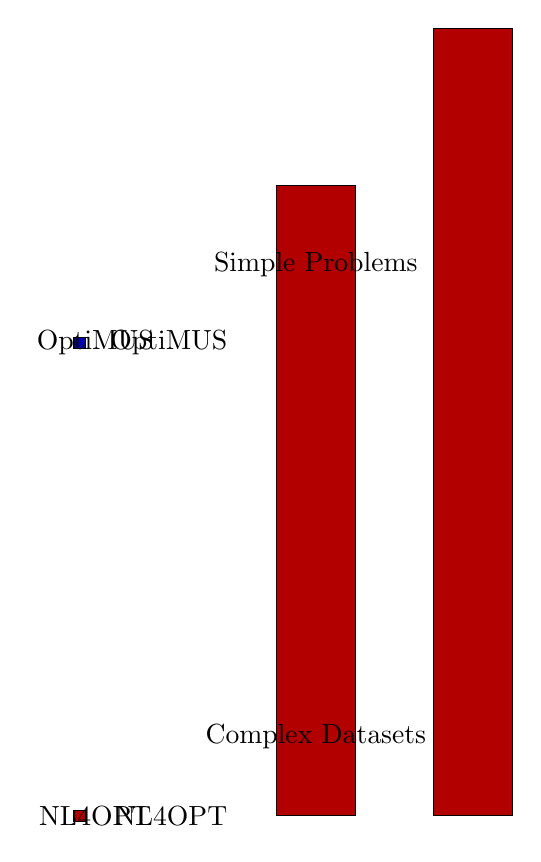
\begin{tikzpicture}[bar width=15pt, y=2cm]
    % Define colors
    \colorlet{optimus}{blue!70!black}
    \colorlet{nl4opt}{red!70!black}

    % Define nodes for the agents
    \node[anchor=east] (Optimus) at (0,0) {OptiMUS};
    \node[anchor=east] (NL4OPT) at (0,-3) {NL4OPT};

    % Draw bars for OptiMUS
    \draw[fill=optimus] (0.5,0) rectangle (1.5,1);
    \draw[fill=optimus] (2.5,0) rectangle (3.5,2);

    % Draw bars for NL4OPT
    \draw[fill=nl4opt] (0.5,-3) rectangle (1.5,1);
    \draw[fill=nl4opt] (2.5,-3) rectangle (3.5,2);

    % Add labels for the bars
    \node at (1,0.5) {Simple Problems};
    \node at (1,-2.5) {Complex Datasets};

    % Add legend
    \node[rectangle, fill=optimus, draw, inner sep=2pt] at (-2,0) {};
    \node at (-1.8,0) {OptiMUS};

    \node[rectangle, fill=nl4opt, draw, inner sep=2pt] at (-2,-3) {};
    \node at (-1.8,-3) {NL4OPT};
\end{tikzpicture}
\end{document}